\section{Ladder Operator Block-Encoding (LOBE)}
\label{sec:lobe}

The block-encodings presented in this work builds off of the constructions of \cite{camps2024explicit} and \cite{liu2024efficient} to provide a more general block-encoding of Hamiltonians described in the form of Eq. \ref{eq:lclo}.
Explicity, the construction presented in this work allows for the terms in the Hamiltonian to be any arbitrary product of ladder operators acting on fermions, antifermions, and bosons.
Additionally, we make use of the observations presented in Subsection \ref{subsec:unification} to provide block-encodings of the same structure as an LCU which have reduced rescaling factors.
This also extends LCU block-encodings to the non-unitary operators used in this work and may provide a framework for constructing block-encodings of linear combinations of other non-unitary operators.

\begin{figure}
    \centering
    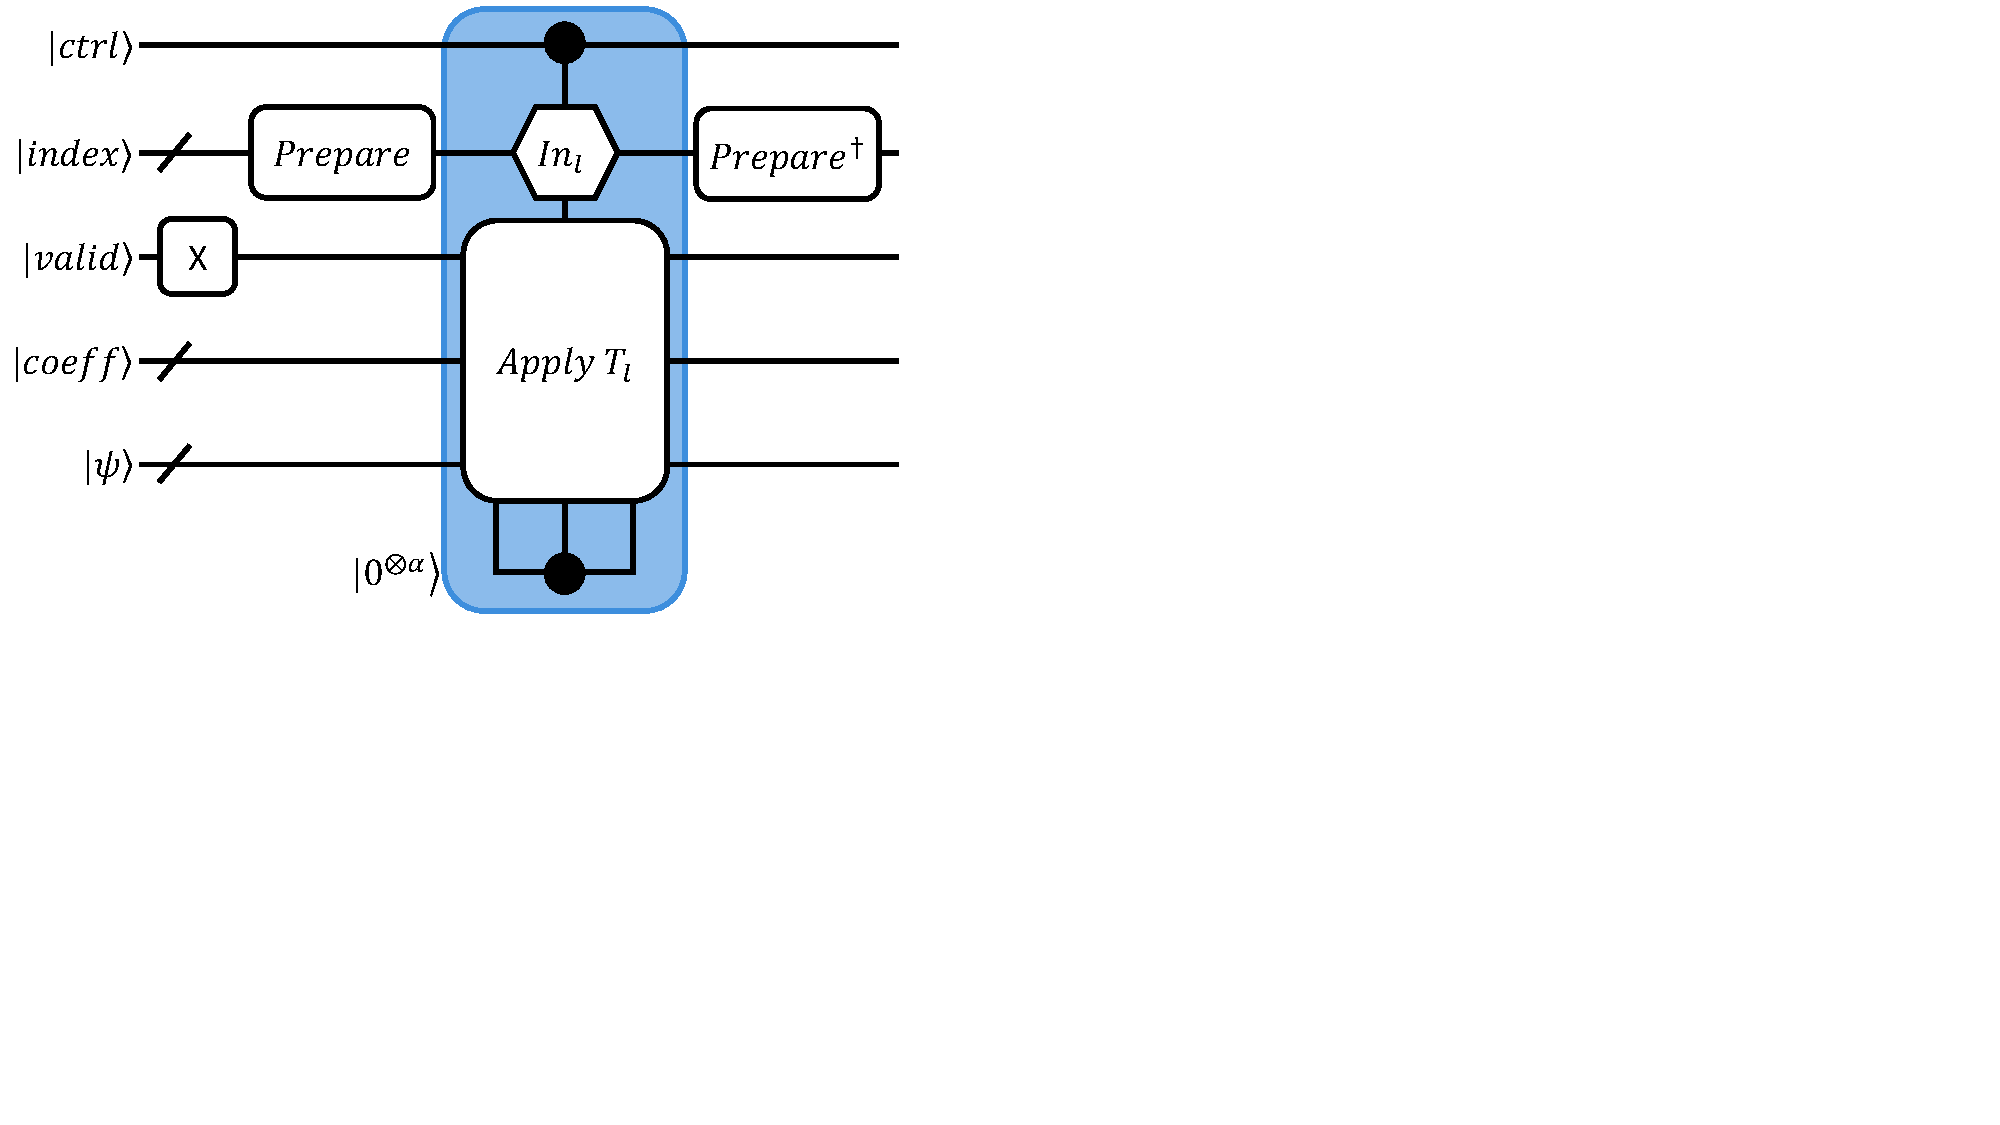
\includegraphics[width=8cm]{figures/lobe.pdf}
    \caption{\textbf{Ladder Operator Block-Encoding.}
    }
    \label{fig:lobe}
\end{figure}

In Figure \ref{fig:lobe}, we define the LOBE circuit in terms of generic oracles.
The LOBE circuit is structured similarly to an LCU circuit in that it involves sequential application of a $\textit{Prepare}$ oracle, a $\textit{Select}$ oracle, and then uncomputing the $\textit{Prepare}$ oracle using the daggered circuit.

There are numerous space-time tradeoffs that one can make to either reduce the number of ancillae qubits at the cost of more gates or vice versa.
In this work, we opt for compilations that minimize the number of non-Clifford operations at the expense of more ancillae qubits.

Since the most costly operations to perform are those that will require preparation of magic states (non-Clifford operations) \ws{Is this only true for surface code?}, the analytical gate counts will be computed in terms of the following non-Clifford operations: (arbitrary rotations, left elbows, right elbows).
For ease, we will express these gate counts as an ordered tuple:
\begin{equation}
    \label{eq:gate-counts}
    C = (N_{\textit{rot}}, N_{\textit{left}}, N_{\textit{right}})
\end{equation}
where left and right elbows are defined by \cite{babbush2018encoding}.

A single left-elbow produced from 2 controls will require 1 clean ancilla qubit and 4 T gates. 
A corresponding right-elbow will require a measurement and a classically conditioned Clifford operation.
As the exact cost of a right elbow will likely be highly dependent on the physical architecture and quantum error-correction scheme, it will be counted independently.
A left-elbow with $N$ controls producing one ancilla qubit storing the quantum boolean can be decomposed into elbows using only 2 controls each, using $N-1$ total ancillae (including the output boolean) with the following cost:
\begin{equation}
    \label{eq:N-ctrl-elbow}
    C_{N-ctrl-elbow} = (0, N-1, N-2)
\end{equation}

Additionally, arbitrary rotations are typically decomposed into non-Clifford operations via one of several methods \cite{}. \ws{Ross-Selinger, RUS, phase gradient states} 
The cost of these decompositions is dependent upon the desired rotation angle and the required precision on the angle of the rotation.
For this reason, we will leave these costs in terms of rotations and elbows instead of decomposing them further into T gates.

\subsection{Qubit Registers}
\label{subsec:registers}

The LOBE circuit makes use of 5 qubit registers: $\ket{\textit{index}}$, $\ket{\textit{valid}}$, $\ket{\textit{coeff}}$, $\ket{\psi}$, and $\ket{0^{\otimes \alpha}}$.
This disregards the control qubit ($\ket{\textit{ctrl}}$) in Figure \ref{fig:lobe} as it is not required for applying an uncontrolled block-encoding.

The register denoted $\ket{\textit{index}}$ is referred to as the index register and is used to index the terms in the Hamiltonian as is done in LCU constructions. 
The integer representations of the computational basis states of the index register corresponds to the indices $l$ in Eq. \ref{eq:lclo}. 
The minimum number of qubits required for the index register is given by:
\begin{equation}
    Q_{\textit{index}} = \lceil \log_2{L} \rceil
\end{equation}

The register denoted $\ket{\textit{valid}}$ consists of a single qubit and is referred to as the validation qubit.
It serves the same purpose as in \cite{liu2024efficient} which is to denote whether or not the term at the current index ($T_l$) should be applied onto the system and if it will annihilate the quantum state.
Suppose the term $T_l$ will annihilate the state based on the occupation of the fermionic and antifermionic modes. 
In that case, the validation qubit remains in the $\ket{1}$ state such that that branch of the wavefunction remains outside the encoded subspace of the block-encoding.
This action on the validation qubit will be described in more detail in Subsection \ref{subsec:select}.
If the term will not annihilate the state, then the validation qubit gets flipped to the $\ket{0}$ state for the term $T_l$.
The validation qubit is initialized in the $\ket{1}$ state which can either be assumed or implemented via a single $X$ gate applied to the $\ket{\textit{valid}}$ qubit once it is initialized.
The single $X$ gate in Figure \ref{fig:lobe} depicts this initialization and is \textit{not} repeated on subsequent applications of the block-encoding.
\ws{Still need to explicitly verify this}

The register denoted $\ket{\textit{coeff}}$ is referred to as the coefficient register and is used to store the coefficients associated with the bosonic ladder operators in term $T_l$. 
% The number of qubits required for the bosonic coefficients is $A$ which is the maximum number of bosonic operators acting within a single term.
If we let $M$ denote the maximum number of bosonic modes with operators acting on them within a single term, then the minimum number of qubits in the coefficient register is given by:
\begin{equation}
    Q_{\textit{coeff}} = M 
\end{equation} 
% If $USP$ is used for preparation of the index register, then an additional qubit is required.
One additional qubit may be required to apply the $\alpha_l$ coefficient depending on the \textit{Prepare} oracle that is used.
% These coefficients include the coefficients associated with the bosonic ladder operators and can also include the coefficients of the terms in the linear combination ($\alpha_l$) depending on the \textit{Prepare} oracle that is used.

The register denoted $\ket{\psi}$ is referred to as the system register and is used to encode the state of the system.
This register can be broken up into three subsequent registers: the fermionic system $\ket{\psi_b}$, the antifermionic system ($\ket{\psi_d}$), and the bosonic system ($\ket{\psi_a}$).
% The encoding studied in this work is outlined in more detail in Subsection \ref{subsec:encoding}.
Using the qubit-efficient encoding described in Subsection \ref{subsec:encoding}, the minimum number of qubits required for the system registers is given by:
\begin{equation}
    \begin{split}
        &Q_{\psi_b} = I \\
        &Q_{\psi_d} = I \\
        &Q_{\psi_a} = I \lceil \log_2{(\Omega + 1)} \rceil \\
        &Q_{\psi} = Q_{\psi_b} + Q_{\psi_d} + Q_{\psi_a} = 2I + I\lceil \log_2{(\Omega + 1)} \rceil
    \end{split}
\end{equation} 

Finally, the register denoted $\ket{0^{\otimes Q_\alpha}}$ is referred to as the clean ancillae register where $Q_\alpha$ will be used to refer to the number of qubits in this register.
This register includes ancillae qubits that are promised to begin in the $\ket{0}$ state and are returned to this state at the end of the block-encoding circuit.
These temporary, clean ancillae are allocated and deallocated as the block-encoding circuit proceeds.
The maximum number of clean ancillae required is dependent upon the exact compilation methods for both \textit{Prepare} and \textit{Select}.

\subsection{Rescaling of Coefficients Due to Bosonic Terms}
\label{subsec:rescaling}

The inclusion of bosonic ladder operators in our models requires rescaling the coefficients of our Hamiltonian such that they are always normalized and appropriately weighted.
As shown in Eqs. \ref{eq:bosonic-creation} and \ref{eq:bosonic-annihilation}, bosonic ladder operators acquire a coefficient on the state that is proportional to the square-root of the occupation of the state.
From these definitions, it is clear that if we were to apply a block-encoding that contains bosonic ladder operators onto a quantum state, the output quantum state may not be normalized.

To remedy this, we can rescale the coefficients that are picked up by the operators such that the states are always normalized.
In the case of bosonic ladder operators, we can rescale Eqs. \ref{eq:bosonic-creation} and \ref{eq:bosonic-annihilation} by dividing by the square-root of the maximum allowable occupation number plus one such that any coefficient acquired is $< 1$:
\begin{equation}
    \label{eq:bosonic-ops-altered}
    \begin{split}
        \Tilde{a}_i^\dagger \ket{n_{a_i}} &= \sqrt{\frac{n_{a_i} + 1}{\Omega + 1}} \ket{n_{a_i} + 1} \hspace{1em} when \ket{n_{a_i}} \neq \ket{\Omega} \\
        \Tilde{a}_i  \ket{n_{a_i}} &= \sqrt{\frac{n_{a_i}}{\Omega + 1}} \ket{n_{a_i} - 1} \hspace{1.7em} when \ket{n_{a_i}} \neq \ket{0}
    \end{split}
\end{equation}
where $\Tilde{*}$ indicates that these operators are now defined to have a different (rescaled) action and we will refer to them as \textit{rescaled} bosonic ladder operators.
We do not redefine these equations for the cases where the state is annihilated since they will be the same as in Eqs.  \ref{eq:bosonic-creation} and \ref{eq:bosonic-annihilation}.
% These rescaled coefficients will be accounted for within the action of the \textit{Select} oracle as described in Subsubsection \ref{subsec:select}.

The overall coefficient of the output state when multiple rescaled bosonic ladder operators are present within a single term ($T_l$) will be rescaled by a factor of:
\begin{equation}
    \lambda_{A_l} = (\Omega + 1)^{A_l/2}
\end{equation}
where $A_l$ is the number of rescaled bosonic operators included in the term $T_l$.

Different terms within the Hamiltonian may have different numbers of bosonic operators and therefore will have differing rescaling factors of $\lambda_{A_l}$.
In order to guarantee that this rescaling is consistent across the different terms, we can classically preprocess the coefficients in the Hamiltonian such that after the block-encoding is applied, all output states have the same bosonic rescaling factor.
If we define $A \equiv \max_l{A_l}$, then we can define the preprocessed coeffieints as:
\begin{equation}
    \label{eq:bosonic-coeff-rescaling}
    \alpha_l \rightarrow \frac{\alpha_l}{(\Omega + 1)^{(A - A_l)/2}} \equiv \tilde{\alpha_l}
\end{equation}
where the coefficients $\tilde{\alpha_l}$ are the rescaled coefficients of the terms.

% This preprocessing means that after the block-encoding is applied, all output states will be rescaled by a coefficient of $(\Omega + 1)^{(A)/2}$.
The \textit{bosonic-rescaled} Hamiltonian is given by:
\begin{equation}
    \tilde{H} = \sum_{l=0}^{L-1} \tilde{\alpha_l} \Tilde{T}_l
\end{equation}
where $\tilde{H}$ is the rescaled Hamiltonian and $\Tilde{T}_l$ refers to the term $T_l$ with the bosonic ladder operators replaced by the rescaled bosonic ladder operators in Eq. \ref{eq:bosonic-ops-altered}.

Overall, the bosonic rescaling factor is given by:
\begin{equation}
    \label{eq:bosonic-rescaling-factor}
    \lambda_A = (\Omega + 1)^{A/2}
\end{equation}
such that the matrix elements of $\tilde{H}$ are the matrix elements of $H$ with a constant rescaling factor:
\begin{equation}
    H_{i,j} = \lambda_A \tilde{H}_{i,j}
\end{equation}

\subsection{Prepare Oracle}
\label{subsec:prepare}

In this work, we discuss two implementations of LOBE that both lead to valid block-encodings of the same Hamiltonians.
These two variations have similar costs in terms of the circuit construction, but potentially significantly different rescaling factors.
The main difference between these two implementations is the application of the coefficients of the terms in the Hamiltonian.

In the variant inspired by the sparse block-encoding approach of \cite{camps2024explicit, liu2024efficient}, the coefficients are loaded within the \textit{Select} oracle.
This variant will use \textit{Uniform State Preparation} for the \textit{Prepare} oracle which is synonymous with the \textit{Diffusion operator} in \cite{camps2024explicit, liu2024efficient}.

In the variant inspired by LCU, the coefficients are loaded with the \textit{Prepare} oracle.
This variant will use \textit{Arbitrary State Preparation} for the \textit{Prepare} oracle.

Below, we will discuss both the cost and the implied rescaling factors of both \textit{Prepare} oracles.
Including this rescaling factor \textit{and} the bosonic rescaling factor (Eq. \ref{eq:bosonic-rescaling-factor}), the overall rescaling of the Hamiltonian that is block-encoded is given by:
\begin{equation}
    \label{eq:post-process}
    H = (\lambda_A * \lambda_{prepare}) \bar{H}
\end{equation}
with $\lambda_{prepare}$ being either $\lambda_{USP}$ or $\lambda_{ASP}$ which are defined below.


\subsubsection{Uniform State Preparation}
\label{subsubsec:usp}

As is done in \cite{camps2024explicit} and \cite{liu2024efficient} using the Diffusion operator, one implementation of the $\textit{Prepare}$ oracle is to create a uniform superposition over the computational basis states of the index register.
This is done using a series of Hadamard gates on each qubit in the register.
We will refer to this variant of the \textit{Prepare} oracle as \textit{Uniform State Preparation} or \textit{USP}.

A condition for this implementation is that the coefficients must first be rescaled such that they all have magnitude $\leq 1$.
Let the largest coefficient magnitude be given by $\alpha^* = \max{|\tilde{\alpha_l}|}$.
This rescaling imposes a constant rescaling factor of $\alpha^*$ and we refer to these rescaled coeffifients as $\Tilde{\alpha_l}$.

\textit{USP} imposes an additional rescaling factor of $2^{\lceil \log_2{L} \rceil}$.
This results in an overall rescaling of the Hamiltonian by a constant factor of:
\begin{equation}
    \label{eq:usp-rescaling}
    \lambda_{prepare} = \lambda_{USP} \equiv 2^{\lceil \log_2{L} \rceil} \alpha^*
\end{equation}
such that the rescaled Hamiltonian is given by:
\begin{equation}
    \label{Hbar scale}
    H = (\lambda_A * \lambda_{USP}) \bar{H}
\end{equation}

The quantum resource requirements of this implementation of $\textit{Prepare}$ are negligible as no ancillae are required and only Clifford operations (Hadamards) are performed.
However, this implementation of $\textit{Prepare}$ requires that the rescaled coefficients of the terms ($\Tilde{\alpha_l}$) be incorporated within the $\textit{Select}$ oracle which will be described in Subsection \ref{subsec:select}.

\subsubsection{Arbitrary State Preparation}
\label{subsubsec:asp}

An alternative implementation of $\textit{Prepare}$ is to use the same implementation traditionally used in LCU circuits which we will refer to as \textit{Arbitrary State Preparation} or \textit{ASP}.

For \textit{ASP}, the rescaling factor is given by the $L1-norm$ of the coefficients:
\begin{equation}
    \label{eq:asp-scale}
    \lambda_{prepare} = \lambda_{ASP} \equiv \sum_{l=0}^{L-1} | \tilde{\alpha_l} |
\end{equation}
and the rescaled Hamiltonian is given by:
\begin{equation}
    H = (\lambda_A * \lambda_{ASP}) \bar{H}
\end{equation}
It should be noted that $\lambda_{ASP} \leq \lambda_{USP}$ with equality when the coefficients of the terms all have equal magnitude.
A proof for this claim is given in Appendix \ref{sec:proof-of-rescaling-factors}.

The goal of \textit{ASP} is to perform the following operation:
\begin{equation}
    \ket{0^{\otimes \lceil \log_2{L} \rceil}} \rightarrow_{\textit{Prepare}} \sum_{l = 0}^{L-1} \sqrt{|\tilde{\alpha}_l| / \lambda_{ASP}} \ket{l}
\end{equation}
This results in a weighted superposition over the computational basis states of the index register.
The squared amplitudes of the basis states are equal to the magnitude of the associated coefficients of the Hamiltonian ($\{\tilde{\alpha}_l\}$).

For Hamiltonians that have structure among the coefficients of the terms, implementations of $\textit{ASP}$ can be constructed that leverage this structure.
In certain cases, this can drastically reduce the cost of $\textit{ASP}$ such as is done for the Fermi-Hubbard model in \cite{babbush2018encoding}.
When a certain structure cannot be assumed, the Grover-Rudolph algorithm from \cite{grover2002creating} gives a formulaic routine to generate \textit{ASP} circuits.

In Appendix \ref{sec:grover-rudolph}, we discuss Grover-Rudolph and the circuit compilation strategy in more detail.
Implementing Grover-Rudolph as described in Appendix \ref{sec:grover-rudolph} incurs the following gate counts:
\begin{equation}
    C_{GR} = (\sum_{i=0}^{\lceil \log_2{L} \rceil - 1} 2^i, 0, 0)
\end{equation}
where $L$ is the number of terms in the Hamiltonian.

\subsection{Select Oracle}
\label{subsec:select}

\begin{figure}
    \centering
    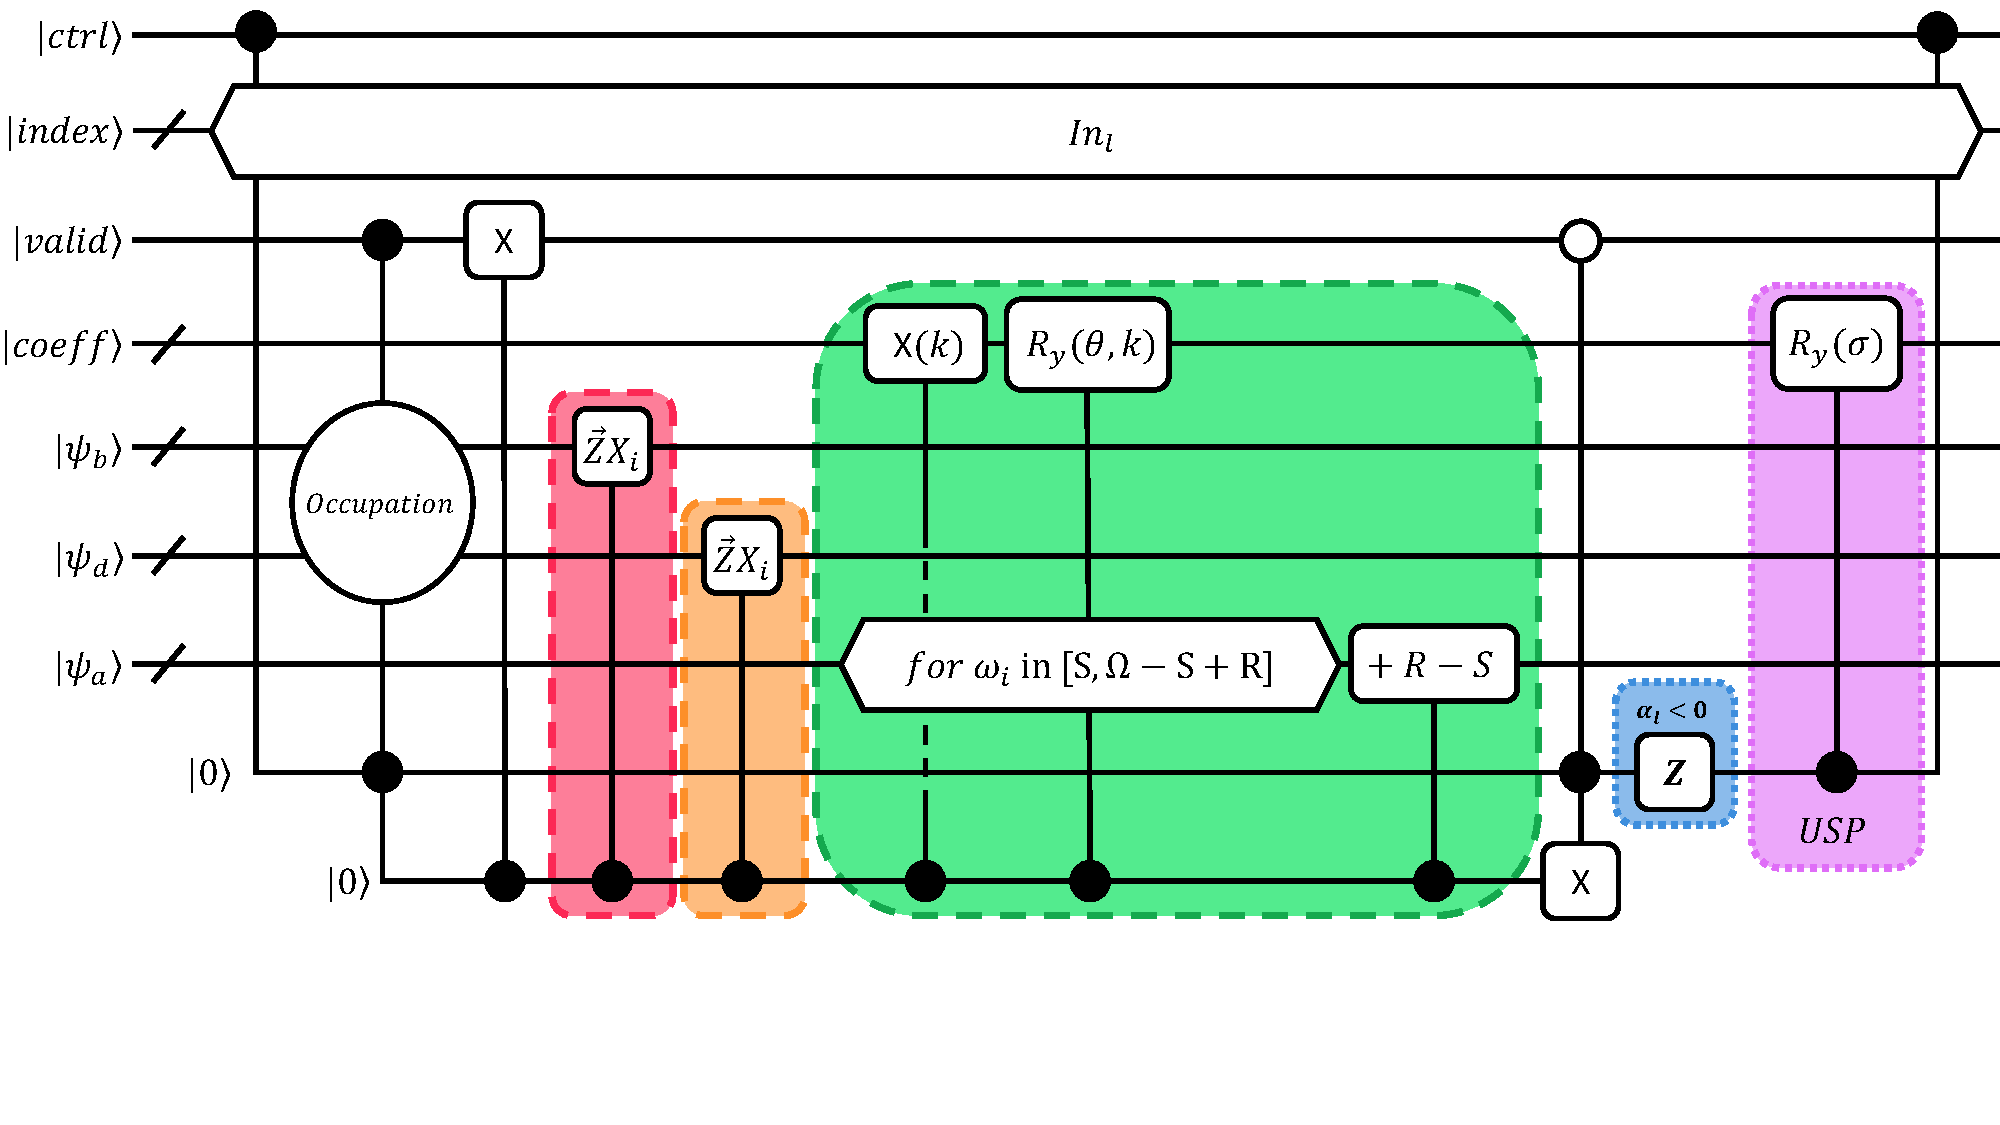
\includegraphics[width=16cm]{figures/select.pdf}
    \caption{\textbf{Ladder Operator Select Oracle (Decomposed).}
    }
    \label{fig:select}
\end{figure}

The \textit{Select} oracle is shown in Figure \ref{fig:lobe} as the oracle within the blue shaded region.
As is done in standard LCU circuits, the \textit{Select} oracle is designed such that it applies the term $T_l$ onto the system when the index register is in the computational basis state $\ket{l}$.
In Figure \ref{fig:select}, we give a circuit diagram for \textit{Select} focusing on the application of a single term, $T_l$.
The \textit{Select} oracle can be constructed by applying the circuit for each term ($T_l$) when the ancilla qubit of the multiplexing operator over the index register is in the computational basis state $\ket{l}$.

Throughout this work, the hexagonal boxes in circuit diagrams will represent multiplexors or coherent for-loops over the computational basis states of the registers on which they are applied..
An explicitly compiled circuit diagram for a controlled multiplexor is given in Figure 7 of \cite{babbush2018encoding} using approximately $L$ left and right elbows and $\lceil \log_2{L} \rceil$ ancillae qubits.
However, for the particular case of multiplexing when the applied unitary at each index is a rotation around the same axis, we use the compilation strategy of \cite{mottonen2004transformation} which is elaborated upon in Appendix \ref{sec:multiplexed-rotations}.

Working from left to right, the first operation shown in Figure \ref{fig:select} is the left-elbow of the controlled multiplexor over the index register.
This puts the ancilla qubit in the $\ket{1}$ state when the index register is in the computational basis state $\ket{l}$.
The gate cost of this controlled multiplexor is approximately:
\begin{equation}
    C_{\text{multiplex: index}} = (0, L, L)
\end{equation}
and requires the following clean ancillae:
\begin{equation}
    Q_{\alpha}^{\text{multiplex: index}} = \lceil \log_2{L} \rceil
\end{equation}

Next, a left-elbow - controlled on the validation qubit being in the $\ket{1}$ state, the index register being in the $\ket{l}$ state (determined by the previous ancilla qubit), and the system being in a state that will not be annihilated - is applied to produce a new ancilla qubit.
This ancilla qubit represents a quantum boolean that determines if the term $T_l$ should be applied onto the system in this branch of the wavefunction without zeroing-out the state.
To perform a check on if the state will be annihilated, controls are added based on the occupation of the fermionic and antifermionic modes corresponding to the operators that are present within the current term.
For each fermionic (antifermionic) creation operator acting on mode $i$, a $0$-control is added on $i^{th}$ fermionic (antifermionic) mode within $\ket{\psi_b}$ ($\ket{\psi_d}$).
Likewise, for each fermionic (antifermionic) annihilation operator acting on mode $i$, a $1$-control is added on $i^{th}$ fermionic (antifermionic) mode within $\ket{\psi_b}$ ($\ket{\psi_d}$).
If both ladder operators are present, then only the $1$-control on the $i^{th}$ mode remains since the state gets zeroed-out only if the mode is unoccupied (assuming that the term is normal ordered).
If any of these conditions are not satisfied, then the state should be zeroed-out and the ancilla qubit will remain in the $\ket{0}$ state for that branch of the wavefunction.
The quantum states that should be zeroed-out due to the bosonic operators will be handled when applying the coefficients of the bosonic operators to the system (green shaded box).

In total, this operation will have $2 + B_l + D_l$ controls for the term $T_l$, incurring the following cost (Eq. \ref{eq:N-ctrl-elbow}):
\begin{equation}
    C_{\text{term-boolean}} = (0, 1 + B_l + D_l, B_l + D_l)
\end{equation}
The maximum number of clean ancillae that will be required for this is:
\begin{equation}
    Q_\alpha^{\text{term-boolean}} = 1 + B
\end{equation}
with all but the output boolean qubit being immediately cleaned after the variable is computed.

After these checks are performed, the bottom ancilla qubit will be in the $\ket{1}$ state if and only if the three conditions are met.
This indicates that the term $T_l$ should be applied onto the system and that the fermionic ladder operators will not zero-out the state.
If the ancilla is in the $\ket{1}$ state, the validation qubit is first flipped from $\ket{1}$ to $\ket{0}$ to put the appropriate branch of the wavefunction into the encoded subspace.
This operation is a Clifford and therefore the gate cost is negligible and no ancillae are required.

The term $T_l$ is then applied to the system registers as portrayed in the shaded boxes with the dashed borders in Figure \ref{fig:select}.
All operations for applying the term $T_l$ (shaded boxes with dashed borders) will be controlled on this ancilla qubit determining if the term should be applied.
We will omit this clarification regarding the control on the following operations from the text for brevity.

The first shaded box (red) in Figure \ref{fig:select} shows the update on the fermionic system corresponding to a single creation or annihilation operator acting on the $i^{th}$ mode.
Since both the creation and annihilation operators flip the occupation and apply a phase - dependent on the parity of the occupation of the preceeding modes - they can both be applied using the same circuit.
To apply the appropriate phase, Pauli $Z$ gates are applied on all the fermionic modes for $j < i$.
To flip the occupation of the mode that the ladder operator acts on, a Pauli $X$ gate is applied to the $i^{th}$ fermionic qubit.
This series of gates is repeated for all fermionic creation or annihilation operators.
Many of these gates could be compiled out of the circuit, however, they are all Clifford operations and therefore will not significantly contribute to the cost of the block-encoding.
The second shaded box (orange) in Figure \ref{fig:select} portays the application of an antifermionic ladder operator and is constructed in an analogous way, but acts on the corresponding antifermionic modes.
All of these operations are Cliffords and likewise we exclude their gate-cost from our analysis.
They also do not require the use of any additional ancillae.

Next, the third shaded box (green) in Figure \ref{fig:select} depicts the action of bosonic ladder operators acting on the $i^{th}$ bosonic mode of the system.
This box is repeated for each bosonic mode that is being acted upon within the current term.
We will define our construction assuming that each term has be normal-ordered, however, we note that the construction presented here can generalize to terms that are not normal ordered with slight modifications.

Let any series of (normal-ordered) bosonic operators acting on the $i^{th}$ mode be described by:
\begin{equation}
    (a_i^\dagger)^R (a_i)^S
\end{equation}
where $R$ and $S$ are nonzero integers in the range $[0, \Omega]$.
The subscripts $*_{l, i}$ will be omitted from $S$ and $R$ in this section for brevity, but are implied.
The action of the rescaled operator on the state of the $i^{th}$ bosonic mode with initial occupation $\omega_i$ is given by:
\begin{equation}
    \label{eq:bosonic-operator-action}
    (a_i^\dagger)^R (a_i)^S \ket{\omega_i} = \prod_{r=0}^{R-1} \big( \sqrt{\frac{\omega_i - S + r + 1}{\Omega + 1}} \big) \prod_{s=0}^{S-1} \big( \sqrt{\frac{\omega_i - s}{\Omega + 1}} \big) \ket{\omega_i + R - S}
\end{equation}

This operation can implemented in the block-encoding via a quantum circuit as follows with $m$ denoting the number of bosonic modes that have already been applied in this term:
\begin{algorithmic}[1]
    \State Let $\ket{\text{fire}}$ be the quantum boolean indicating that the term $T_l$ should be applied onto the quantum state if $\ket{\text{fire}} == \ket{1}$.

    \For{$\ket{m} \in [0, M-1]$}

        \If{$\ket{\text{fire}} == \ket{1}$}
            \State Apply a Pauli-X gate on the $m^{th}$ qubit in the coefficient register to rotate it completely outside of the encoded subspace.
            \For{Multiplex: $\omega_i \in S \leq \omega_i \leq \min(\Omega, \Omega - S + R)$}
                \State Apply an Ry rotation on the $m^{th}$ qubit in the coefficient register of angle $\theta$ given by Eq. \ref{eq:smarter-rot-angle}
            \EndFor

            \State $\ket{\omega_i} \gets \ket{\omega_i + R - S}$
        \EndIf
    \EndFor
\end{algorithmic}
For the multiplexor over the occupation states, any state beginning with an occupation less than $S$ will be zeroed-out and therefore can be left outside of the encoded subspace by setting the rotation angle to zero.
Likewise, any state that should \textit{end} with an occupation greater than $\Omega$ will also be zeroed-out and therefore can also be left unmodified by setting the rotation angle to zero.
For occupation states inside the allowable range, the purpose of the rotations is to rotate the $m^{th}$ qubit in the coefficient register back into the encoded subspace with an amplitude in the $\ket{0}$ state equal to the amplitude in Eq. \ref{eq:bosonic-operator-action}:
\begin{equation}
    \label{eq:smarter-rot-angle}
    \theta(\omega_i, S, R) = 2 \sin^{-1}{\Big(\prod_{r=0}^{R-1} \big( \sqrt{\frac{\omega_i - S + r + 1}{\Omega + 1}} \big) \prod_{s=0}^{S-1} \big( \sqrt{\frac{\omega_i - s}{\Omega + 1}} \big)\Big)}
\end{equation}
The implementation for these controlled-multiplexed rotations is discussed in more detail in Appendix \ref{sec:multiplexed-rotations}.
The gate cost for one of these controlled-multiplexed rotations is given by:
\begin{equation}
    \begin{split}
        C_{\text{bosonic-multiplex-rotations}} &= (2 + 2^{\lceil \log_2(\Omega) \rceil}, 2^{\lceil \log_2(\Omega) \rceil}, 2^{\lceil \log_2(\Omega) \rceil}) \\
        &\approx (2 + \Omega, \Omega, \Omega)
    \end{split}
\end{equation}
and requires one additional clean ancilla qubit that is immediately cleaned.
% \begin{equation}
%     Q_\alpha^{\text{bosonic-multiplex-rotations}} = 1
% \end{equation}

The update of the occupation states is implemented via a controlled-quantum addition operation that is discussed in Appendix \ref{sec:addition}.
With the classical value that is added being $+ R - S$, this contributes a gate cost of:
\begin{equation}
    C_{+ R - S} = (0, \lceil \log_2{\Omega + 1} \rceil - p - 1, \lceil \log_2{\Omega + 1} \rceil - p - 1)
\end{equation}
with $p$ determined by the binary representation of $+ R - S$ as described in Appendix \ref{sec:addition}.
This operation also requires $2(\lceil \log_2{\Omega + 1} \rceil - p) - 1$ clean ancillae which are immediately cleaned after the operation.
% \begin{equation}
%     Q_\alpha^{+ R - S} = 2(\lceil \log_2{\Omega + 1} \rceil - p) - 1
% \end{equation}

Since these operations are repeated $M_l$ times for the term $T_l$, the total gate cost is given by:
\begin{equation}
    C_\text{bosonic-updates} \approx \sum_m (2 + \Omega, \Omega + \lceil \log_2{\Omega + 1} \rceil - p_m - 1, \Omega + \lceil \log_2{\Omega + 1} \rceil - p_m - 1)
\end{equation}
and a number of clean ancillae upper-bounded by:
\begin{equation}
    Q_\text{bosonic-updates} \leq 2 \lceil \log_2{\Omega + 1} \rceil - 1
\end{equation}
% This operation can implemented in the block-encoding via a quantum circuit as follows with all operations controlled on the ancilla qubit indicating if the current term should be applied, with $k$ denoting the number of bosonic modes that have already been accoutned for in this term:
% \begin{enumerate}
%     \item Apply a Pauli-X gate on the $k^{th}$ qubit in the coefficient register to rotate it completely outside of the encoded subspace.
%     \item Multiplex over the occupation of the $i^{th}$ bosonic mode for occupation states in the range: $S \leq \omega_i \leq \min(\Omega, \Omega - S + R)$. Any state beginning with an occupation less than $S$ will be "zeroed-out" and therefore can be left outside of the encoded subspace without any additional operations. Likewise, any state that should \textit{end} with an occupation greater than $\Omega$ will also be "zeroed-out" and therefore can also be left unmodified.
%     \item For each value of $\omega_i$ in the multiplexor, apply a rotation on the $k^{th}$ qubit in the coefficient register of angle $\theta$ given by Eq. \ref{eq:smarter-rot-angle}. The purpose here will be to rotate the qubit back into the encoded subspace with an amplitude in the $\ket{0}$ state equal to the amplitude in Eq. \ref{eq:bosonic-operator-action}. 

%     \begin{equation}
%         \label{eq:smarter-rot-angle}
%         \theta(\omega_i, S, R) = 2 \sin^{-1}{\Big(\prod_{r=0}^{R-1} \big( \sqrt{\frac{\omega_i - S + r + 1}{\Omega + 1}} \big) \prod_{s=0}^{S-1} \big( \sqrt{\frac{\omega_i - s}{\Omega + 1}} \big)\Big)}
%     \end{equation}

%     \item Update the occupation by a value of $+ R - S$. If $R = S$, no update is needed.
% \end{enumerate}
% Overall, this requires one multiplexor and one qubit in the coefficient register for each bosonic mode that is being acted upon within the term.
% The multiplexors will also have a reduced number of occupation modes to multiplex over, thereby reducing the number of Toffolis required for each multiplexor.

Once the state of the system is updated and the bosonic coefficients have been applied, the bottom ancilla qubit can be uncomputed (reset to $\ket{0}$).
This can be achieved by applying a Toffoli onto this qubit with a zero-control on the validation qubit and a one-control on the ancilla qubit used for multiplexing over the index register.
This Toffoli gate can be decomposed into one pair of elbows using one ancilla qubit that is immeidately cleaned:
\begin{equation}
    C_{\text{clean: term-boolean}} = (0, 1, 1)
\end{equation}
\ws{It's not quite clear to me if we can use a right-elbow here instead of a Toffoli since we are changing the states of fermionic/antifermionic modes after the left-elbow. Obviously it's only one Toff so it's not a big deal, but I wanna try to do some derivations for this.}

Next, if the sign of the coefficient of the current term is $-1$, we apply a $- \mathds{1}$ - controlled on the index register being in the state $\ket{l}$ - to the state, regardless of which \textit{Prepare} oracle is used.
This operation is shown in the fourth shaded box (blue) with the dotted border to indicate that this operation may or may not be present depending on the sign of the term.
This can be achieved in many ways, but here we simply use a Pauli-Z gate acting on the ancilla qubit storing the state of the multiplexor acting on the index register.
This is only Clifford gates and does not require any ancillae.

Finally, if the \textit{uniform state perparation} protocol is used for the \textit{Prepare} oracle, then the normalized coefficient of the term must be applied.
This is achieved via a controlled Pauli-Y rotation that is applied onto the final qubit in the coefficient register (this is the qubit that does not get touched by the bosonic updates).
This is shown in the fifth shaded box (purple) with the dotted border to indicate that this operation may or may not be present depending on which \textit{Prepare} oracle is used.
This rotation is used to account for the rescaled coefficient of the term ($\Tilde{\alpha_l}$) and is achieved by applying a rotation with an angle given by:
\begin{equation}
    \sigma(\Tilde{\alpha_l}) \equiv 2 \cos^{-1}{|\Tilde{\alpha_l}|}
\end{equation}
If the \textit{arbitrary state preparation} protocol is used, then this rotation is not needed as the coefficient of the term is already accounted for and one fewer qubit is needed in the coefficient register.
A controlled rotation may be perfomed with two rotations and two CNOT gates, thereby incurring the following cost:
\begin{equation}
    C_{\Tilde{\alpha_l}}^\text{USP} = (2, 0, 0)
\end{equation}
where the $*^\text{USP}$ superscript indicates that this cost is only included when \text{USP} is used for \textit{Prepare}.

In total, the approximate number of clean ancillae required is given by:
\begin{equation}
    \begin{split}
        Q_\alpha &= 2 + \lceil \log_2{L} \rceil + \max{(2 \lceil \log_2{\Omega + 1} \rceil - 1, B, 1)} \\ 
    \end{split}
\end{equation}
where $2$ ancillae are used to store the quantum booleans in Figure \ref{fig:select}, $B$ are temporarily used for computing the ``term-boolean'', $2 \lceil \log_2{\Omega + 1} \rceil - 1$ are temporarily used for the update of the bosonic occupancy, $1$ is temporarily used in many of the operations such as the controlled-multiplexed rotations and the Toffoli to reset the quantum boolean.
Under the assumption that $2 \lceil \log_2{\Omega + 1} \rceil - 1 > B > 1$, the maximum number of ancillae required is given by:
\begin{equation}
    Q_\alpha \approx 1 + \lceil \log_2{L} \rceil + 2 \lceil \log_2{\Omega + 1} \rceil
\end{equation}

The total qubit requirement under these compilation choices - disregarding the control qubit and the optional qubit required when $USP$ is used - is given by:
\begin{equation}
    \begin{split}
        Q &= Q_{\textit{index}} + 1 + Q_{\textit{coeff}} + Q_{\psi_b} + Q_{\psi_d} + Q_{\psi_a} + Q_\alpha \\
        &\approx \lceil \log_2{L} \rceil + 1 + M + 2I + I\lceil \log_2{(\Omega + 1)} \rceil + 1 + \lceil \log_2{L} \rceil + 2 \lceil \log_2{\Omega + 1} \rceil \\
        &\approx 2(\lceil \log_2{L} \rceil) + (I + 2)\lceil \log_2{(\Omega + 1)} \rceil + 2I + M + 2
    \end{split}
\end{equation}
which is linear in the number of modes and logarithmic in the number of terms and the bosonic occupation cutoff.

For the overall gate counts, we will focus on the variant using Grover-Rudolph to implement \textit{ASP}, however it is straightforward to compute the associate gate counts for $\text{USP}$.
Beginning from Figure \ref{fig:lobe}, we can compute the overall gate cost of the block-encoding as $2*C_{GR} + C_{\textit{Select}}$.
$C_{\textit{Select}}$ can be computed as a sum of the individual costs outlined above:
\begin{equation}
    \begin{split}
        C_{\textit{Select}} &= C_{\text{multiplex: index}} + \sum_l (C_{\text{term-boolean}} + C_\text{bosonic-updates} + C_{\text{clean: term-boolean}}) \\
        &\begin{split}
            &\approx (0, L, L) \\
            &+ \sum_l (0, 1 + B_l + D_l, B_l + D_l) \\
            &+ \sum_l \sum_m (2 + \Omega, \Omega + \lceil \log_2{\Omega + 1} \rceil - p_m - 1, \Omega + \lceil \log_2{\Omega + 1} \rceil - p_m - 1) \\
            &+ \sum_l (0, 1, 1) \\ 
        \end{split} \\
    \end{split}
\end{equation}
Though the exact gate counts are not clear from this expression, we can see that the asymptotic gate counts are given by:
\begin{equation}
\begin{split}
    N_\text{rot} &= O(LM \Omega) \\
    N_\text{elbow} &= O\big(L + LI + LM(\Omega + \log{\Omega}) \big)
\end{split}
\end{equation}
where $M$ is upper-bounded by $I$.

% Since the $\textit{Prepare}$ oracle for $USP$ is simply a string of Hadamard gates, this oracle contributes no non-Cliffords and $C_{\textit{USP}} = (0, 0, 0, 0)$.
% In Appendix \ref{sec:grover-rudolph}, we discuss the gate cost for the implementation of Grover-Rudolph used in this work. \ws{Fill this out once gate cost is better understood.}

% For the cost of the $\textit{Select}$ oracle, we will focus on the form when using $USP$ for $\textit{Prepare}$.
% When Grover-Rudolph is used instead, the only change to the $\textit{Select}$ oracle is that the controlled rotation is not included and therefore the rotation count is reduced accordingly.  

% The cost of the controlled-multiplexor over the index register is given by $L - 1$ left (and right) elbows \cite{babbush2018encoding} where $L$ is the number of terms in the Hamiltonian or the number of computational basis states we are interested in.
% This accounts for the cost of generating the quantum boolean second from the bottom in Figure \ref{fig:select}.
% No rotations or additional Toffolis are required, therefore the cost is given by: 
% \begin{equation}
%     C_{\textit{index}} = (0, 0, L-1, L-1)
% \end{equation}

% The rest of the gate cost of the $\textit{Select}$ oracle can be computed as the sum of the cost of implementing the individual terms:
% \begin{equation}
%     C_{\textit{Select}} = C_{\textit{index}} + \sum_{l} C_{T_l}
% \end{equation}

% The first operation performed for each term is the computation of the bottom qubit in Figure \ref{fig:select}.
% This quantum boolean is computed via a left-elbow with $B_l + D_l + 2$ controls where $B_l$ and $D_l$ represent the number of fermionic and antifermionic modes being acted upon within the term $T_l$.
% As was mentioned in Subsubsection \ref{subsubsec:space}, this multi-controlled operation can be decomposed into $B_l + D_l + 1$ left elbows and $B_l + D_l$ right elbows.

% Flipping the validation qubit and performing the fermionic and antifermionic operators only require Cliffords and therefore do not contribute to the gate counts we are interested in.

% Next, we have the cost of implementing the bosonic operators.
% For each of the $M_l$ bosonic modes being acted upon within the term $T_l$, we must perform a controlled-multiplexor over the $\Omega - 2S_{l, m} + R_{l, m}$ non-trivial occupation states of the mode being acted upon.
% Where $l$ indexes the term in the Hamiltonian and $m$ indexes the bosonic mode being acted upon within the $l^{th}$ term.
% This will require $\Omega - 2S_{l, m} + R_{l, m} - 1$ left (and right) elbows and for each nontrivial occuptation state, a controlled rotation will be performed.
% Therefore, we can sum up the cost of implementing all of the $M_l$ bosonic operators as: 
% \begin{equation}
%     C_{M_l} = \Big(\Sigma_l, 0, \Sigma_l - M_l, \Sigma_l - M_l \Big)
% \end{equation}
% where $\Sigma_{l} \equiv \Omega - 2S_{l, m} + R_{l, m}$.

% \ws{Add cost of adding classical values to bosonic registers here. Will cost a decent number of Toffolis.}

% Uncomputing the bottom ancilla qubit requires one Toffoli. \ws{still not sure if this can be replaced by a right-elbow.}
% Lastly, when $USP$ is used for $\textit{Prepare}$, a controlled rotation is performed.
% Therefore, the overall cost of implementing a single term \ws{temporarily neglecting the cost of incrementing/decrementing} is given by:
% \begin{equation}
%     C_{T_l} = \Big(1 + \Sigma_l, 1, B_l + D_l + 1 + \Sigma_l - M_l, B_l + D_l + \Sigma_l - M_l \Big)
% \end{equation}

% Therefore, the overall cost of implementing the $\textit{Select}$ oracle is given by:
% \begin{equation}
%     \begin{split}
%     C_{\textit{Select}} &= C_{\textit{index}} + \sum_{l} C_{T_l} \\
%     &= \Big(L + \sum_l \Sigma_l, L, 2L - 1 + \sum_l \big( B_l + D_l + \Sigma_l - M_l \big), L-1 + \sum_l \big( B_l + D_l + \Sigma_l - M_l \big)\Big)
%     \end{split}
% \end{equation}
